\chapter{Theoretical Background and Related Work}
\label{chapter:background} 

In chapter \ref{chapter:intro} a brief general analysis of stereo geometry and methods has been provided. 
In this chapter a more precise revision of the theoretical tools that stereo matching methods exploit is presented.
Epipolar geometry, camera calibration and disparity estimation algorithms are specifically described. 
Starting from the necessary mathematical basis, the discussion moves on the disparity estimation algorithms. 
Then, the chapter focus on the main benefits and drawbacks of standard and novel approaches in depths computation.
Comparison between stereo-geometry based and deep learning based algorithms is proposed, to provide a clear explanation of the decisions implemented. 

\section{Epipolar geometry and Rectifiation}
\label{sec:eipolarandrect}

Fundamental problem of stereo vision is the estimation of 3D locations of points from at least two corresponding input images.
This process, which comprises concurrent computation of both 3D geometry and camera pose, is generally known as structure from motion \cite{Szeliski2011}.\\
In the explanation of these topics it is necessary to start discussing about the triangulation.
Then, the concept of epipolar geometry is outlined and after that the notions of camera calibration and rectification. 

\subsection{Triangulation}
\label{subsec:triangulation}

\begin{figure}[t]
	\begin{center}
		{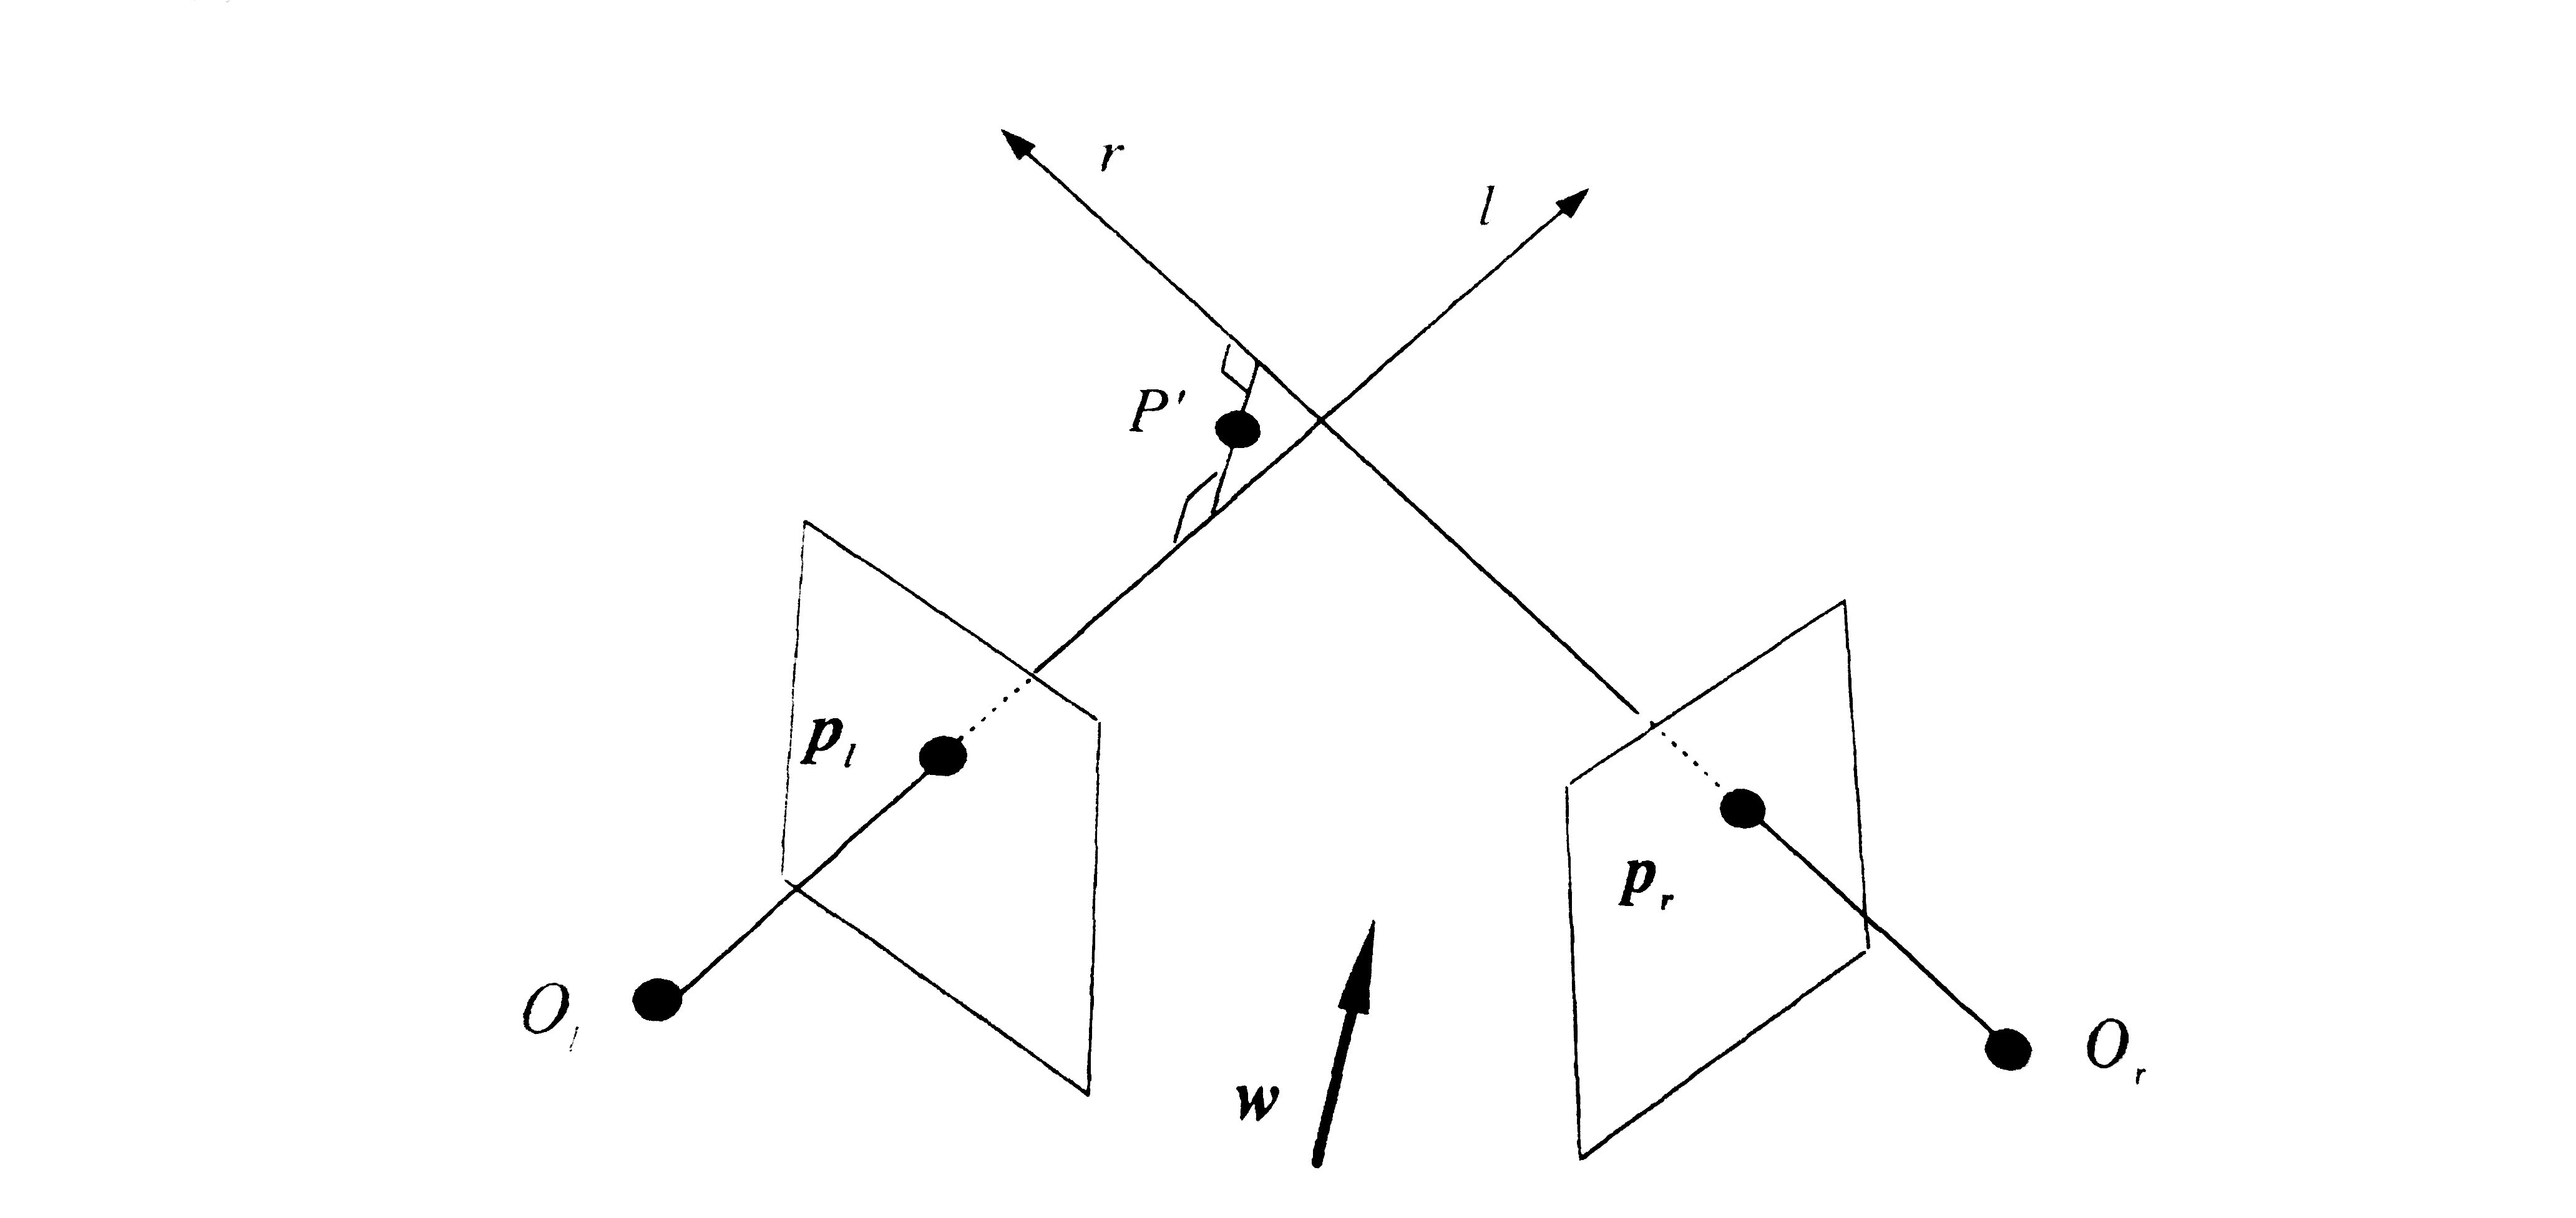
\includegraphics[width=.8\textwidth]{images/triangulation}}
\caption{3D triangulation by finding point $P'$ that lies nearest to all of the optical rays}
\label{fig:triangulation}
	\end{center}
\end{figure}

Triangulation is the problem of detecting 3D points positions from a collection of corresponding 2D image locations, assuming that camera positions are known.
Figure \ref{fig:triangulation} shows one of the easiest methods to tackle this problem. 
Objective is to evaluate the 3D position of $P'$ that have the smallest error to all of the 3D optical rays coming from the camera centers, which identify the 2D point locations in the image plane, i.e. $P_r$ and $P_l$.
As shown in Figure \ref{fig:triangulation}, the rays starts from the camera centers, $O_j$ and go in direction of $r$ and $l$, which can be defined using the camera matrix $ \{ P_j = K_j [ R_j | t_j ] \} $.
The closest point to $P$ on this ray minimizes the distance
\begin{equation}\label{eqn:mindist}
	\Vert O_j + d_j \hat{v}_j - P \Vert^2
\end{equation}
Therefore, because of the minimum is $d_j = \hat{v}_j \cdot (p - c_j)$, the nearest points are calculated as:
\begin{equation}\label{eqn:closestpoint}
	q_j = O_j + (\hat{v}_j \hat{v}_j^\top)(P - O_j) = O_j + (P - O_j)_{\Vert}
\end{equation}
Hence, the optimal value for $P$, obtained solving a least square problem, becomes,
\begin{equation}\label{eqn:solP}
	P = \Big[ \sum_j (I - \hat{v}_j \hat{v}_j^\top ) \Big]^{-1} = \Big[ \sum_j (I - \hat{v}_j \hat{v}_j^\top )O_j \Big]
\end{equation}

\subsection{Epipolar geometry}
\label{subsec:epipolargeom}

\begin{figure}[t]
	\begin{center}
		{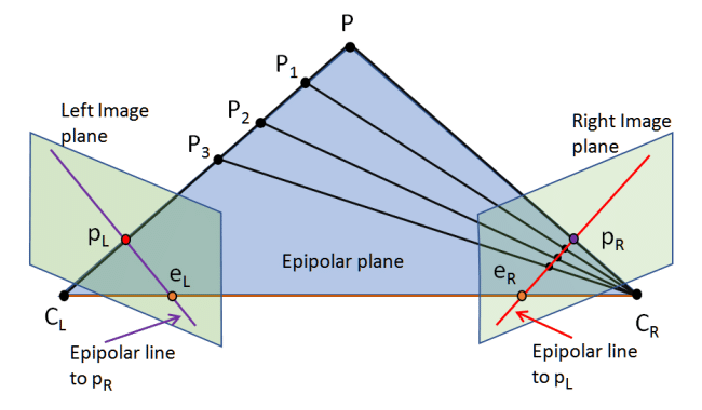
\includegraphics[width=.8\textwidth]{images/epipolar-geometry-2}}
\caption{Epipolar geometry. Image point $m$ back-projects to a ray in a 3D space defined by $C$ and $m$. This ray becomes a line $l'$ in the second view. The image of $X$ must lie on $l'$}
\label{fig:epipolargeom-2}
	\end{center}
\end{figure}

The intrinsic projective geometry between two views is known as epipolar geometry.
It is only dependent on the cameras' internal parameters and pose.
The $3 \times 3$ rank 2 matrix that defines this geometry is the fundamental matrix $F$.\\
The epipolar geometry is the basis for finding corresponding points in stereo matching. 
It is basically defined by the intersection between image planes and the one on which the cameras baseline lies.\\
A fundamental property, that makes this geometry extremely useful, is that image points, space point and camera centers are coplanar. 
Assuming that only $m_l$ is known, that geometry allows to constraint the corresponding point $m_r$. 
The epipolar plane is defined by the baseline and the ray that comes from $m_l$. 
Hence, knowing that $m_r$ lies on the same plane, that point belongs to $l_r$, i.e. the intersection between the epipolar and the second image plane. 
Therefore, exploiting this property, the searching of corresponding points is constrained to only one line inside the image.\\
Mathematical definition of the epipolar geometry is the fundamental matrix $F$.
As already demonstrated through Figure \ref{fig:epipolargeom-2}, for each point $p_L$ in one image, the corresponding epipolar line $e_R$ to that point belongs to the other image plane. 
Moreover, any point $p_R$ in the second image, which is related to point $p_L$, lies on $e_R$.
Hence, the epipolar line is described as the projection in the second image of the ray that comes from the point in the first image, passing through its camera center.
This defines a map, $p_L \rightarrow e_R$, which relates the points in one image with the corresponding epipolar lines in the second image.
This correlation, between points and lines, is represented by the fundamental matrix $F$.\\
Considering the aforementioned map $p_L \rightarrow e_R$ described by $F$, an important property of the fundamental matrix is defined,
\begin{equation}\label{eqn:fundmatprop}
	p_R^\top F p_L = 0
\end{equation}
Therefore, assuming two corresponding points $P_L$ and $p_R$, it is known that $p_R$ lies on the epipolar line $l_R = F p_L$. 
Thus, the mathematical correlation is,
\begin{equation}
	0 = p_R^\top e_R = p_R^\top F p_L
\end{equation}
Reciprocally, if image points comply the relation \ref{eqn:fundmatprop}, then the rays identified by these points are coplanar. 
For point corresponding this is a necessary condition.
Equation \ref{eqn:fundmatprop} is extremely important because it allows to characterize the fundamental matrix without reference to the camera matrices \cite{hartley2004multiple}.
Thus, using at least 7 correspondences, it is possible to recover the fundamental matrix $F$. 
This estimation is known as \textit{weak calibration}.\\
\textbf{Maybe add 8-point algorithm description}

\subsection{Rectification}
\label{subsec:rectification}

Image rectification is defined as the process of obtaining a pair of \textit{matched epipolar projections} from a pair of stereo images, which are taken from generally differing viewpoints.
In the rectified projections the epipolar lines become parallel with respect to the x-axis. 
Thus, they match between the stereo pair and so the disparities are in the x-direction only.\\
In order to obtain a rectified stereo pair, 2D projective transformations are employed to the images, so that the epipolar lines can match.
Using this method, the transformations are built up in a way that the corresponding points have almost the same x-coordinate.
Actually, this strategy leads to a minimal distortion on the images, being the two transformations arbitrary. 
However, working on rectified images, the matching problem is highly simplified, being correlated only to epipolar geometry and near-correspondence. \\
Core problem of this section is to find the appropriate projective transformation $H$. 
Indeed, to get epipolar lines parallel with x-axis, the epipole should be mapped to an infinite point. 
This, has to be done correctly, otherwise intensive projective distortion of the image can happen.
For this reason, constraints are put on the definition of $H$.\\
First of all, restricting $H$ to be a rigid transformation in the neighbourhood of a given point\footnote{this means that to first-order, the neighbourhood of the point may be subjected to rotation and translation only}, the errors are reduced.\\
Once the epipole has been mapped to infinity, it is then necessary define a map to match the corresponding epipolar lines.
This resampling is build up in such a way that, being $e_L$ and $e_R$ any pair of epipolar lines, then,
\begin{equation}
	H^{-\top} e_L = H'^{-\top} e_R
\end{equation}
Satisfying the condition above, a matched pair of transformations is recovered.\\
Specifically, at first $H'$ is chosen, so that it can map the epipole $e_R$ to infinity. 
Then the matching transformation $H$ is defined minimizing the sum-of-square distances,
\begin{equation}\label{eqn:matchtransfconstr}
	\sum_i d(H p_{L_i}, H'p_{R_i})^2
\end{equation}

Therefore, the full algorithm can be summarized as follows.\\
The outcome of this resampling process is a pair of stereo images whose epipolar lines are horizontal.
Hence, the disparities are calculated along the epipolar lines. 
First of all, at least seven corresponding matches are defined.
This allows to compute the fundamental matrix $F$, applying the so called eight-point algorithm, and after that the two epipoles are found.
After that, there is the selection of the projective transformation $H'$, that maps the epipole of the support image to infinity.
The corresponding transformation $H$ is found solving the least-square problem.
Finally both of the input images are resampled according to $H$ and $H'$.

\section{Stereo methods and dense correspondence}
\label{sec:stereometh}

\textbf{Take the part already written in the introduction}\\
\textbf{Refactoring needed between the 2 chapters}

\subsection{Stereo geometry based methods}

\subsection{Deep learning based methods}
\label{subsec:deeplearnmeth}

Considering that disparity estimation from a rectified stereo pair is still one of the most important tasks in computer vision, the latest years have seen an important development of deep learning based methods. \\
Usually these approaches comprises a main pipeline, based on a standard local or global method, whose parameters are finely tuned exploiting Convolutional Neural Networks (CNNs). 
Therefore, in most of the cases, Semi Global Matching (SGM) is used as regularization method, because of its accuracy and low computational time. 
Then, deep learning based methods are used for tuning the penalty parameters, which are related to smoothness and discontinuity of the disparity map. 
As described above, those penalties are empirically adjusted in the standard methods. 
Therefore, the CNNs based approach aims at learn the penalties, in correlation with the 3D structure of the objects in the scene, to achieve an improvement in the disparity map. \\
As aforementioned, several of these deep learning approaches has been proposed in the latest years, and some of them has been able to reach state of the art level of accuracy on the KITTI datasets.\\
Even though these method suffer drop in accuracy when shifting from synthetic to real images, it is worth to describe some of them, which are ranked among the state of the art methods in the KITTI benchmark. \\
Seki and Pollefeys proposed SGM-Nets\cite{Seki2017}, a CNNs based method for penalty estimation, which exploit SGM as regularization technique in the main pipeline. 
They used small image patches and their locations as inputs to the network to predict penalties for the 3D object structures. 
Actually, they developed a novel loss function for training the networks, which inputs are small image patches and their position. 
Moreover, they managed to separate positive and negative disparity changes, thus to get object structures more discriminatively.\\
More in detail, SGM-Net produces $P_1$ and $P_2$ for each pixel. 
This is achieved though a training and a testing phase. 
In the former, the network is iteratively trained by minimizing a \textit{Path cost} and a \textit{Neighbor Cost}. 
In testing, the standard SGM pipeline is run using the penalties estimated by the network. 
Actually, the \textit{Path Cost} is how the authors of the paper called the loss function that they developed, which they minimized using forward and back propagation. 
Moreover, they introduced the \textit{Neighbor cost} function for removing the ambiguous disparities traversed along along the path, which can lead to wrong penalties.\\
Another approach similar to the one just described is the method developed by Kuzmin et al. \cite{Kuzmin2017}. 
The core of their method is the prediction of the local parameters of cost volume aggregation process, which they perform exploiting a deep convolutional network. 
Thus, as in \cite{Seki2017}, they avoid to apply deep learning of pixel appearance descriptors, using classical matching scores instead. 
Thus, they refuse learning high dimensional descriptors and matching them, as it used to happen in most of the first deep learning based algorithm.
On the contrary, they focus the learning on the cost-aggregation step. 
Thus, they defined the overall matching cost using a combination of census transform and sum-of-absolute-differences. 
Then, they carry out the cost-aggregation phase, which is peculiar for smoothing the general matching cost and correct the wrong matches, applying the domain transform \cite{Gastal2011},\cite{Pham2013}.
Basically, they develop a deep convolutional neural network to estimate on a pixel basis the cost-aggregation parameters and make them spatially varying. 
In this way, they were able to have smoother disparities on the same object and avoid smoothing across object boundaries. 
Therefore, combining standard methods for the matching cost and applying end-to-end deep learning process to the cost-aggregation step, they obtain state-of-the-art accuracy in the KITTI 2015 dataset. 
Differently from \cite{Zbontar2016}, \cite{Zbontar2015} and similarly to \cite{Mayer2016}, they build up an end-to-end learning method that comprises all the part of depth map computation in it. 
Furthermore, unlike \cite{Mayer2016}, their approach exploits classical stereo matching techniques as modules within a more complex neural network structure. 
Their process encompasses the definition of a general cost volume, the cost-aggregation step over that volume and the final winner-takes-all label selection. 
Then, left-right consistency and filling of occluded pixels are performed as post-processing.\\
A different approach with respect to the previous one stands in the implementation developed by \^{Z}bontar and LeCun \cite{Zbontar2016}.
They focus their attention on the matching cost computation, which is usually the first step of a stereo matching algorithm. 
They developed their method using a convolutional neural network to learn similarity measures on small image patches. 
Specifically, they structure the training in a supervised manner building up a binary classification data set with examples of similar and dissimilar pairs of patches. 
Moreover, they carry out two different architectures, one adjusted for speed, and another one for accuracy. 
Thus, the output of the network handles the initialization of the stereo matching cost. 
After that, post processing steps are applied: cross-based cost aggregation, semi-global matching and finally disparity refinement techniques such as, left-right consistency check, subpixel enhancement, median and bilateral filters.\\
Technically speaking, they present a convolutional neural network that is trained on pairs of small image patches, for which the disparity value is known. 
Then, they initialize the matching cost using the output of the network.
After that, they propose a series of common post-processing steps, which are though crucial to obtain accurate results.
Cross-based cost aggregation is exploited for combining matching cost between neighbouring pixels with similar intensities. Then, constraints are enforced for smoothness and left-right consistency check applied for detect and eliminate errors in occluded regions. 
The final disparity map is then obtained applying median and bilateral filters, useful for subpixel enhancement. \\
Related problems to \cite{Zbontar2016} are the works by Haeusler et al. \cite{Haeusler2013} and by Spyropoulos et al. \cite{Spyropoulos2014}. 
Using a similar approach, they concentrate their attention on predicting the confidence of the calculated matching cost. 
Specifically, in the first cited approach \cite{Haeusler2013}, the aim was using a random forest classifier to connect multiple confidence measures. 
Similarly, the authors of \cite{Spyropoulos2014} focused in estimating the confidence of the matching cost by training a random forest classifier. 
Then, they employed the predictions as mild constraints in a Markov Random Field (MRF) aiming at reducing the errors of the stereo method.\\
Focusing on confidence prediction intended at the estimation of dense disparity map, it is worth to cite the work of \cite{Seki2016}.
They adopted two channels disparity patches as inputs of a Convolutional Neural Network (CNN), predicting the correctness of stereo correspondences, that is the confidence. 
Using these specific patches, they managed to simultaneously train features and classifiers.
Furthermore, they incorporate the predicted confidence into Semi-Global Matching (SGM), adjusting its parameters directly. \\
Unlike methods based on hand crafted features, which lead to limited accuracy, authors of \cite{Seki2016} leverage CNNs to overcome that problem. 
In fact, CNNs support high performance from low level processing, such as patch based matching, to high level, like scene classification and object detection. \\
Therefore, as previously introduced, they conceive a two channels disparity patch, based on the concept of standard confidence features.
Then they apply those patches as input to the network, obtaining a simultaneous training of discriminative features and classifiers.
Moreover, they also developed three different types of network structures to manage the trade-off between computational time and accuracy. 
Finally, the confidence was combined into SGM, so that dense disparity map could be obtained. \\

\subsubsection{Confidence measures}

Considering some of the deep learning based methods described in \ref{subsec:deeplearnmeth}, becomes necessary to define the main typology of features proposed during the years to estimate the confidence of stereo correspondences. \\
Because of many features were introduced by different works in computer vision field, Hu and Mordohai \cite{Hu2012} developed a broad evaluation of them, leading to the definition of five groups, used for categorize those features. \\
The first group is correlated to the matching cost. 
This means that correct correspondence are unlike to be connected to large matching costs. 
The second group focuses on local properties of the cost curve. 
That is, confidence measure becomes the curvature around the minimum matching cost. 
For example, flat curves, which have smaller values, and describe texture-less areas express higher ambiguity.
Features related to local minima of the cost curve form the third group. 
As an example, the so called \textit{Peak Ratio (PKR)}, is calculated as the minimum matching cost divided by the second local minima.
Then, a probability mass function over disparity defined using the entire cost curve describes the fourth group.
The last group includes features that highlight the consistency between left and right disparity map, i.e. correct matches indicate more consistent disparity.\\
A similar but more recent work is the one carried out in \cite{Poggi2017} driven by the deep breakthrough lately happened in computer vision field. 
In fact, changing such as, availability of bigger and more challenging datasets, novel and more accurate stereo algorithms and confidence measures, leverage techniques based on deep learning.
Therefore, the authors of \cite{Poggi2017} focus on implement a complete and updated quantitative analysis of the state-of-the-art confidence measures.\\
As a matter of fact, after the analysis performed in \cite{Hu2012}, major improvements have happened in computer vision field.
Among those the most relevant can be summarized as follows:
\begin{itemize}
	\item enhanced confidence prediction algorithms based on deep learning \cite{poggi2016learning} and on random-forests \cite{Spyropoulos2014}, \cite{Park2015};
	\item larger dataset providing challenging indoor and outdoor scenes \cite{Mayer2016};
	\item more accurate stereo algorithms and novel implementation of the SGM pipeline \cite{Seki2016}, \cite{Zbontar2016}
\end{itemize}
Therefore, in \cite{Poggi2017}, the authors extend and update the taxonomy previously performed in \cite{Hu2012}, especially focusing on machine learning techniques.
Then they aim at evaluating the algorithms' performance over the novel and larger datasets, concentrating on the correlation between the availability of training data and the correctness of confidence measure prediction. 
Moreover, they estimate the accuracy of the methods when handling new data and calculate the effectiveness of the predictions when included in state-of-the-art pipelines.\\
Considering that among the multiple confidence measures proposed, all of them deal with the cost curve and the relationship between left and right image or disparity map, basing on \cite{Hu2012}, Poggi et al. \cite{Poggi2017} grouped confidence measures according to their input cues. 
Specifically, they considered 76 confidence measures, which were then grouped into 8 categories and evaluate them employing three state-of-the-art stereo algorithms and three ground truth datasets: Middlebury 2014 \cite{Scharstein2014}, KITTI 2012 \cite{geiger2013vision} and KITTI 2015 \cite{menze2015object}.
Performing that exhaustive analysis, the authors carried out the results that learning based approaches seem to be more efficient than conventional ones. 
Especially, using disparity maps as input cue more accurate results are achieved in terms of correct matches, adaptation to new data and stereo accuracy improvement. 
Beside that, training remains an issue for those methods though. 
As a matter of fact, for deep learning based approaches the general amount of training data is still limited and in most case they struggle when dealing with new real data.\\


\section{Image processing techniques}
\label{section:image-proc-technique}

In almost all the computer vision methods image processing technique are applied in different phases of the algorithm pipeline in order to model the image in a form convenient for subsequent analysis. 
Image processing stage is a key component of most of the computer vision applications, such as object recognition, stereo matching, computational photography, scene reconstruction, 3D pose recognition or motion flow, in order to achieve reasonable results. 
Different types of processing operations are usually applied, depending on the type of task demanded.
For example commonly applied procedures includes exposure correction, color balancing, noise reduction, smoothness enhancement, sharpness increasing or feature detection.\\
In relation to this Master's thesis project, it is worth to focus on some of those operations, which result to be most relevant for the designed algorithm. 
Especially, point operators, area-based and global image transform techniques will be analysed. 
Particularly, neighborhood (area based) operators will receive specific attention, being the ones specifically employed in the developed algorithm. \\

\subsection{Point operators}
\label{subsection:point-operators}

Point operators are defined as the simplest type of image processing transforms \cite{Szeliski2011}.
For these operators the output pixel value is entirely related to the corresponding input pixel value.
Brightness and contrast adjustment, or color correction and transformation represents some of those techniques.\\
Basically, an image processing operator is identified, in the continuous domain, by the following function that takes one or more input images and generates a corresponding output:
\begin{equation}
 \label{eqn:img-operator}
 g(x) = h(f(x)) \quad 	\mbox{or} \quad g(x) = h(f_0(x), ..., f_n(x))
\end{equation}
where $x$ is in the D-dimensional domain of the functions and $f$ and $g$ operate over some range.
Specifically, for discrete images, the domain comprises a finite number of pixel locations, i.e. $x = (i, j)$, so that:
\begin{equation}
	g(i, j) = h(f(i,j))
\end{equation}
Among these pixel-based operators it is sufficient to cite color transforms, image matting and histogram equalization. 
Therefore, considering color images as arbitrary vector-valued functions, it is coherent to identify them as highly correlated signals with strong connections to the image formation process. \\
Taking into account particular image editing application, where for example the goal is to take a foreground object from a scene and to put it into a different background.
The first step of this processing is called matting, that is cut of a specific object from scene. 
Whereas, the second part, the positioning over a different background is defined compositing.\\
Histogram equalization is, rather, a more widely exploited technique. 
This algorithm is based on the histogram of the individual color channels and luminance values.
Thus, using information about minimum, maximum and average intensity values of the image it is possible to equalize the pixel intensity value of the whole image, that is identify the intensity mapping function $f(I)$ such that the resulting histogram is flat. 

\subsection{Neighborhood operator}
\label{subsection:neighbor-operator}

Differently from the previous type of operators, in this case the output pixel value is evaluated on the basis of its neighboring pixel values.
This category of operators is usually applied for local tone adjustment, but more specifically for multiple kinds of image filtering, such as blurring, sharpening, feature detection or noise removal.
Considering these local transforms, it is important to distinguish between linear and non-linear filtering operators.\\
Linear operators are the most generally used in terms of are-based operators. 
They relate weighted combinations of pixels in a neighborhood in order to estimate the output pixel's value. 
Basically, they can be described by the following function:
\begin{equation}
 \label{eqn:local-linear-oper}
 g(i, j) = \sum_{k,l} f(i + k, j + l)h(k, l)
\end{equation}
where the entries in the weight kernel $h(k, l)$ are called \textit{filter coefficients}.
More simply, the relation \ref{eqn:local-linear-oper} can be written as:
\begin{equation}
	\label{eqn:compact-loc-lin-op}
	g = f \otimes h
\end{equation}
An important mention has to be done in relation to the separable filters.
As a matter of fact, when filters are applied to a 2D image and convolution is taken into account, that requires $K^2$ operations per pixels, i.e. multiplication and summation, defining $K$ as the kernel size.
In most cases, the filtering process can be accelerated carrying out a one-dimensional horizontal convolution and subsequently a vertical convolution. 
This procedure requires, in fact, only $2K$ operations per pixels.
However, this cannot be always done, but it can be applied only to the convolution kernels that are said to be \textit{separable}. \\
The proof of that property for a convolution kernel can be achieved by inspecting at its analytic form, as shown in \cite{Freeman1991}.
More precisely that can also be checked handling the 2D kernel as a 2D matrix $\mathbf{K}$ and taking its singular value decomposition (SVD), as follows:
\begin{equation}
	\label{eqn:svd-check-separable}	
	\mathbf{K} = \sum_{i} \sigma_i \mathbf{u}_i \mathbf{v}_i^\top
\end{equation}
Therefore, it is proved that if only the first singular value $\sigma_0$ is non-zero, the kernel is separable and $\sqrt{\sigma_0}u_0$ and $\sqrt{\sigma_0}v_0^\top$ give the vertical and horizontal kernels respectively \cite{Szeliski2011}.
Among linear filters, there are some that are commonly used for pre and post processing operations over images, which were tested in this project too.\\
The moving average or box filter is regarded as the simplest one. 
It basically performs a convolution over the image with a kernel of all ones and the result is then scaled. 
The bilinear kernel is, instead, a specific version of the \textit{Bartlett} filter. 
Actually, the bilinear filter is the outer product of two linear splines.\\
Useful kernel for accurate noise removal are the \textit{Gaussian} kernels.
As the operators introduced previously, they are example of low-pass kernels, whose effect is softening higher frequencies, which are correlated with the noise components of the signals\footnote{In the Fourier frequency-space the noise appears to be a high frequency signals}. \\
Taking into account the non-linear filters, they are usually exploited when dealing with the need of achieve more accurate results with respect to the outcome given by linear operators.
Moreover, on top of that, there are the morphological operators, which are neighborhood kernels working with binary images.\\
Focusing on the non-linear operators, some of them has been employed in the designed of this project, in particular in the image pre-processing step of the main pipeline and in the post-processing phase.
Among all the available non-linear area-based kernels, it worth to mention the applied ones.\\
The median filter is one of these. 
Basically, it takes the median value from each pixel's neighborhood.
This kind of filter becomes quite performing when dealing with shot noise, which is difficult to be removed if applied a standard Gaussian kernel.
However, moderate computational cost and the fact that it modify the values pixel-wise are drawbacks of this filter, which has to be taken into account.
For this reason, a \textit{weighted} median filter can be implied, instead. 
In this case, each pixel of the subregion is counted a different number of times depending on its distance from the center.
Therefore, this can be equivalently formulated as the minimization of the weighted objective function:
\begin{equation}
	\label{eqn:weighted-median-filt}
	\sum_{k, l} w(k,l) \vert f(i + k, j + l) - g(i, j) \vert^{p}
\end{equation}
where $g(i,j)$ is the requested output value and $p = 1$ for the weighted median. \\
Besides its heavier computational cost, compared to the linear filtering, non-linear noise removing operators are usually preferred because of their more accurate \textit{edge preserving} capability. 
Hence, when cleaning away noisy frequencies, they tend to soft less the edges.\\
\begin{figure}[t]
	\begin{center}
		{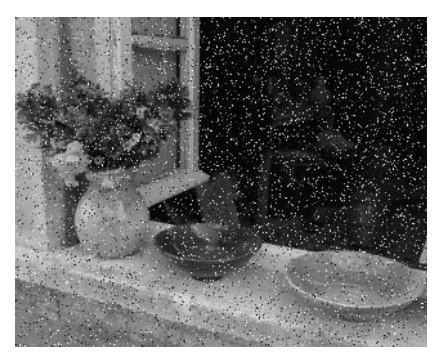
\includegraphics[width=.8\textwidth]{images/filter-example-original-shot-noise.png}}
\caption{Original test image for filter comparison. Shot noise is added on top of the image. Credits \cite{Szeliski2011}}
\label{fig:filter-example-original}
	\end{center}
\end{figure}

\begin{figure}[t]
	\centering
	\subfigure[Gaussian filtered test image]{
 		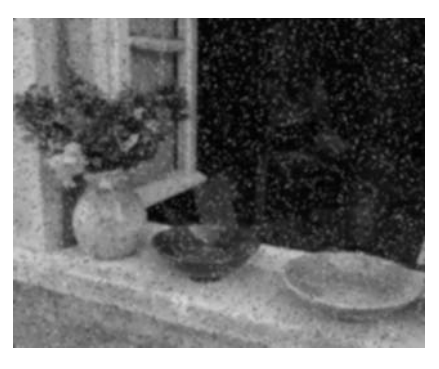
\includegraphics[width=0.4\textwidth]{images/filter-example-gaussian.png}
 		\label{fig:gaussian-filt}
}
	\subfigure[Median filtered test image]{
 		 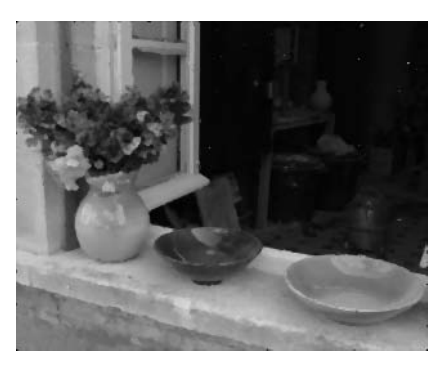
\includegraphics[width=0.4\textwidth]{images/filter-example-median.png}
 		 \label{fig:median-filt}
}
\caption{Test images example taken from \textit{Computer Vision: Algorithms and Applications} \cite{Szeliski2011}}
\label{fig:filter-image-example}
\end{figure}

Figure \ref{fig:filter-example-original} shows a test image where shot noise is added.
Thus, as visible in Figure \ref{fig:filter-image-example}, the Gaussian filter, trying to cancel most of the noise, tends to flatten high-frequency details, which are localized close to strong edges.
Contrarily to the result in Figure \ref{fig:gaussian-filt}, the median filter, shown in Figure \ref{fig:median-filt}, is more edge preserving.\\
Hence, the median filter was chosen in the initial part of the pipeline of this project for the image pre-processing phase, especially for its capability of preserving the edges, without, then, smoothing away the discontinuities.\\
Bilateral filtering is another type of non-linear operator, which was tested during the development of the designed algorithm.
Basically, during the image pre-processing implementation this specific kernel was one of the analysed options.
In fact, it is one of the most common option for noise cancelling in computer vision algorithm.
technically speaking, in the bilateral filter, the value of each transformed pixel is a weighted combination of its neighboring pixel values, as defined by the following equality:
\begin{equation}
	\label{eqn:bilateral-filter}
	g(i, j) = \frac{\sum_{k,l} f(k,l)w(i,j,k,l)}{\sum_{k,l}w(i,j,k,l)}
\end{equation}
where the coefficient $w(i,j,k,l)$ is correlated to the multiplication between a +textit{domain kernel}, defined in equation \ref{eqn:domain-kernel}, and a data-based \textit{range kernel}, illustrate by equation \ref{eqn:range-kernel}.
\begin{equation}
	\label{eqn:domain-kernel}
	d(i,j,k,l) = \exp \Big( - \frac{(i - k)^2 + (j - l)^2}{2 \sigma^2_d} \Big)
\end{equation}
\begin{equation}
	\label{eqn:range-kernel}
	r(i,j,k,l) = \exp \Big( - \frac{\Vert f(i,j) - f(k,l) \Vert^2}{2 \sigma^2_r} \Big)
\end{equation}
Therefore, the \textit{bilateral weight function} can be finally expressed as:
\begin{equation}
	\label{eqn:bilateral-weight-fnct}
	w(i,j,k,l) = \exp \Big( - \frac{(i - k)^2 + (j - l)^2}{2 \sigma^2_d}  - \frac{\Vert f(i,j) - f(k,l) \Vert^2}{2 \sigma^2_r}\Big)
\end{equation}
An unavoidable drawback of the bilateral filter is closely correlated to its computational time, if compared to regular separable filter.
For this reason, as outlined in \cite{Szeliski2011}, multiple acceleration methods have been developed during the last decade.
Nonetheless, those algorithms are prone to a higher memory used w.r.t. the regular filtering, thus they should not be applied to full-color image filtering.\\
A last family of non-linear operators that should be introduce in this chapter consists of morphological filters.
Regarding the designed algorithm, morphological operators have been actually implemented in the post-processing phase in order to remove small estimation error in the 3D point cloud, enhancing the final dense depth 3D reconstruction of the scene.\\
From a theoretical point of view, \textit{morphological operations} are typically implemented over binary or thresholded images. 
This kind of filtering techniques are executed by first convolving the input image with a binary structuring element, which could have different shapes, and after that the result value is defined basing on the outcome of the convolution.\\
If a binary image $f$ is considered and $s$ is the morphological kernel, the convolution operation is defined as:
\begin{equation}
	\label{eqn:morph-convol}
	c = f \otimes s
\end{equation}
where $c$ is the number of 1s inside each structuring element when shifting through the image.
Therefore, designating $S$, the kernel size, the principal morphological operations, which has been tested in the post-processing phase of the algorithm pipeline, comprise:
\begin{itemize}
	\item \textbf{dilation: } $\mathit{dilate}(f,s) = \theta(c, 0)$
	\item \textbf{erosion: } $\mathit{erode}(f,s) = \theta(c, S)$
	\item \textbf{opening: } $\mathit{open}(f,s) = \mathit{dilate}(\mathit{erode}(f, s), s)$
	\item \textbf{closing: } $\mathit{close}(f,s) = \mathit{erode}(\mathit{dilate}(f, s), s)$
\end{itemize}

\section{Edge detection and segmentation algorithms}
\label{section:edge-detect}

Strictly correlated to the latter family of non-linear operation analysed and to the overall performance of the designed algorithm there is the concept of edge detection.\\
Techniques for finding object boundaries in an image are extremely relevant in computer vision and especially when dealing with stereo matching and disparity estimation. 
As a matter of fact, object borders coincide with occlusion points in 3D, where the majority of wrong matches takes place in depth estimation. 
Moreover, segmentation methods are strongly related to this topic and remarkably useful in the preparatory phase of an accurate stereo matching algorithm.\\
Specifically to this work, segmentation techniques have not been completely developed.
This was due to the fact that the initial data provided by the laser points grid already gives a good amount of information for obtaining an accurate 3D dense disparity map.
Beside that, after the evaluation of the first reasonable results obtained, further improvements of the algorithm has been considered to enhance smoothness and continuity among the estimations.
Thus, edge detection and segmentation methods appear to be effective initial operations for multiple reasons, such as, reducing the computational time of the entire pipeline and increasing accuracy and density of the final estimations.\\
Therefore, it is worth to present a brief but sufficient theoretical outline of the most common algorithms designed in the computer vision area, considering that they will be part of the future improvements, which will be applied to work developed so far. \\




\section{Data and estimations error types}
\label{section:error-types}













